\documentclass[12pt]{report}
\usepackage{setspace}  %use this package to set linespacing as desired
\usepackage{array}
\usepackage{graphicx}
\usepackage{subcaption}
\usepackage{amsmath}
\usepackage[counterclockwise, figuresleft]{rotating}

\begin{document}
\doublespacing

\clearpage
\chapter{Results}

\section{Correlation of Parameters}

We observe correlation between two parameters using the statistical definition of the correlation coefficient ($\rho_{X,Y}$), defined as

\begin{equation}
\rho_{X,Y} = \dfrac{cov(X,Y)}{\sigma_X\sigma_Y}
\end{equation}

where \textit{cov} represents covariance. The correlation coefficient is unit-less, and measured from -1.0 $<$ $\rho_{X,Y}$ $<$ 1.0. A correlation coefficient of 0 means the variables X and Y are uncorrelated, while -1.0 means the variables are perfectly inversely correlated; likewise, a correlation coefficient of 1.0 means X and Y are perfectly correlated. Correlation coefficient is used to estimate an environmental parameter's potential usefulness for calculating a new \textit{coneR1} for use in an arbitrary environment.

\subsection{\textit{coneR1} and Average Attenuation} \label{section:coner1andatten}

Both attenuation models (dB and \%$\Delta$) were considered for correlation against optimal \textit{coneR1} values. Results for both are visualized below (Figure \ref{fig:corr_db} and Figure \ref{fig:corr_rgb}). Visualization demonstrates that while correlation coefficient describes the relationship of the two sets (optimal \textit{coneR1} and attenuation) at a superficial level, it cannot describe any translation that may be needed between the two sets.

% dB correlation
\begin{figure}
  \centering
  \begin{subfigure}{1\linewidth}
  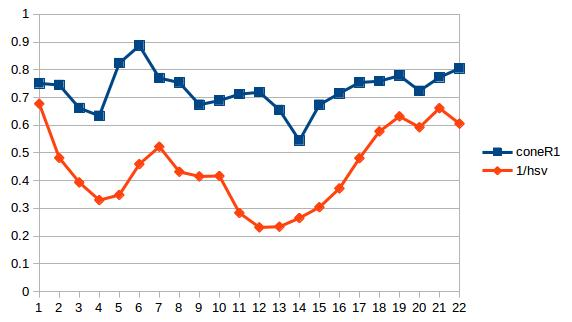
\includegraphics[width=1\linewidth]{figures/correlations/db/room_hsv.jpg}
  \caption{}
\end{subfigure}
\hfill
\begin{subfigure}{.49\linewidth}
  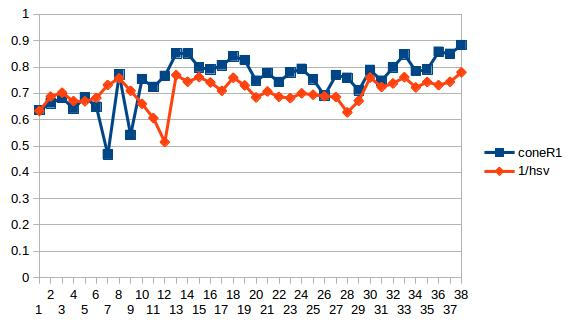
\includegraphics[width=1\linewidth]{figures/correlations/db/campus_hsv.jpg}
  \caption{}
\end{subfigure}
\begin{subfigure}{.49\linewidth}
  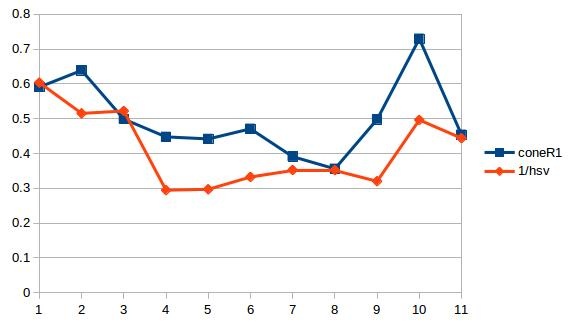
\includegraphics[width=1\linewidth]{figures/correlations/db/pets2_hsv.jpg}
  \caption{}
\end{subfigure}

\caption{Visualization of the correlation discovered between the average attenuation (dB model) of dark shadow pixels, and the \textit{coneR1} algorithmic parameter. All results can be found in the appendix.}
\label{fig:corr_db}
\end{figure}

Tables \ref{table:corr_db} and \ref{table:corr_rgb} present correlation coefficients for each dataset for the dB model and \%$\Delta$ models of attenuation. The variance of both sets of correlated data is included as additional information, to better illustrate the relationship between the sets. For example, while sets of similar variance trend towards higher correlation coefficients, a dataset such as aton\_highway3 may have a high correlative factor despite dissimilar variances; such anomalies indicate non-correlative data points within a set are due to uncharacteristic spikes in either set, rather than a general trend of disassociation. \textbf{Should I include another table detailing translations?}

% Table Form (dB)
\begin{table}
\begin{tabular}{ |c|c|c|c| }
	\hline
	\textbf{Dataset} & \textbf{$\sigma_{coneR1}$} & \textbf{$\sigma_{dB}$} & \textbf{$\rho$} \\
	\hline
	\hline
	\textbf{PETS1} & 0.0007626288 & 0.0077973863 & 0.1985540659 \\
	\hline
	\textbf{PETS2} & 0.0122116182 & 0.0116703923 & 0.6705816077 \\
	\hline
	\textbf{aton\_highway1} & 0.0008668393 & 0.0002027128 & 0.683685054 \\
	\hline
	\textbf{aton\_highway3} & 0.0303058095 & 0.0028347791 &  0.7424117824 \\
	\hline
	\textbf{aton\_room} & 0.0052297835 & 0.0195673253 &  0.5477587003 \\
	\hline
	\textbf{aton\_campus} & 0.0076132319 & 0.0027009857 &  0.3599691597 \\
	\hline
	\textbf{aton\_hallway} & 0.0066428333 & 0.0043961721 &  0.6561589554 \\
	\hline
	\textbf{aton\_lab} & 0.0090227253 & 0.0169701728 &  0.6954036581 \\
	\hline
\end{tabular}
\caption{Datasets and their correlations to \textit{coneR1} (dB model).}
\label{table:corr_db}
\end{table}

% RGB model
\begin{figure}
  \centering
  \begin{subfigure}{1\linewidth}
  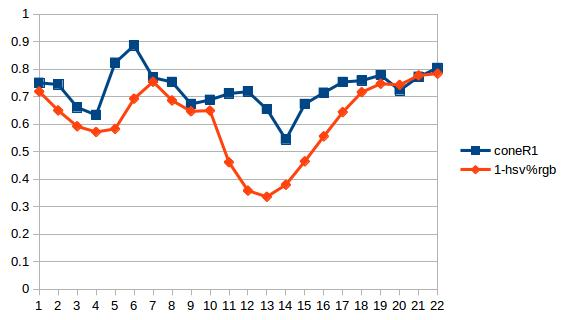
\includegraphics[width=1\linewidth]{figures/correlations/rgb/room_hsv.jpg}
  \caption{}
\end{subfigure}
\hfill
\begin{subfigure}{.49\linewidth}
  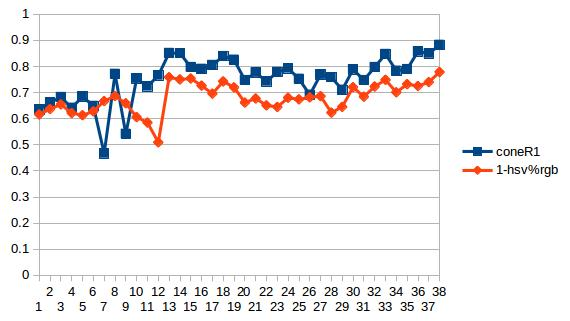
\includegraphics[width=1\linewidth]{figures/correlations/rgb/campus_hsv.jpg}
  \caption{}
\end{subfigure}
\begin{subfigure}{.49\linewidth}
  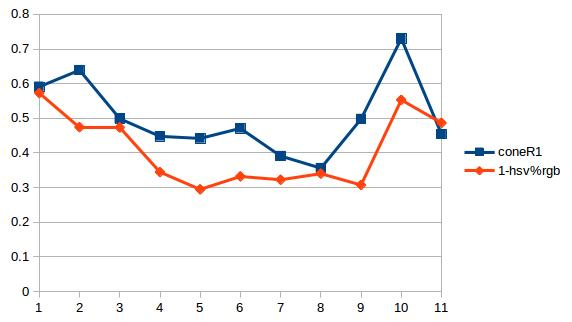
\includegraphics[width=1\linewidth]{figures/correlations/rgb/pets2_hsv.jpg}
  \caption{}
\end{subfigure}

\caption{Visualization of the correlation discovered between the average attenuation (\%$\Delta$ model) of dark shadow pixels, and the \textit{coneR1} algorithmic parameter. All results can be found in the appendix.}
\label{fig:corr_rgb}
\end{figure}

% Table Form (RGB)
\begin{table}
\begin{tabular}{ |c|c|c|c| }
	\hline
	\textbf{Dataset} & \textbf{$\sigma_{coneR1}$} & \textbf{$\sigma_{\%\Delta}$} & \textbf{$\rho$} \\
	\hline
	\hline
	\textbf{PETS1} & 0.0007626288 & 0.0090468985 & 0.1837705578 \\
	\hline
	\textbf{PETS2} & 0.0122116182 & 0.0107841927 & 0.7430874979 \\
	\hline
	\textbf{aton\_highway1} & 0.0008668393 & 0.0001015477 & 0.5923176614 \\
	\hline
	\textbf{aton\_highway3} & 0.0303058095 & 0.0057112872 &  0.8013856844 \\
	\hline
	\textbf{aton\_room} & 0.0052297835 & 0.0189008913 &  0.6226957045 \\
	\hline
	\textbf{aton\_campus} & 0.0076132319 & 0.003236383 &  0.5645999518 \\
	\hline
	\textbf{aton\_hallway} & 0.0066428333 & 0.0041696658 &  0.6897315501 \\
	\hline
	\textbf{aton\_lab} & 0.0090227253 & 0.011644154 &  0.5508747537 \\
	\hline
\end{tabular}
\caption{Datasets and their correlations to \textit{coneR1} (\%$\Delta$ attenuation model).}
\label{table:corr_rgb}
\end{table}

Both the dB and \%$\Delta$ attenuation models are visualized, the better contrast the trends of each method of calculation. Direct qualitative comparison is found in Figure \ref{fig:corr_compare}. 

The results in Tables \ref{table:corr_db} and \ref{table:corr_rgb} indicate that some datasets benefit from the dB attenuation model, while others benefit from the \%$\Delta$ attenuation model. \textbf{Due to the rational nature of the dB calculation,  some data points are exaggerated, increasing correlation within some environments, and decreasing it in others.(awkward?)}

% Compare RGB to dB
\begin{figure}
\centering
\begin{subfigure}{.49\linewidth}
  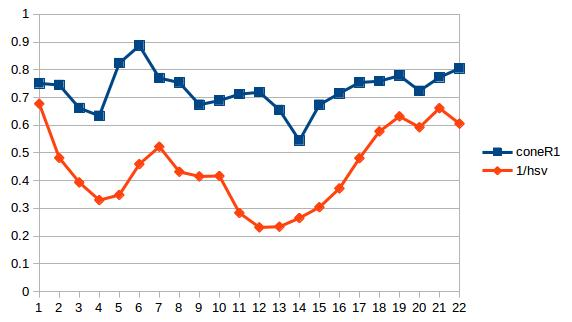
\includegraphics[width=1\linewidth]{figures/correlations/db/room_hsv.jpg}
  \caption{}
\end{subfigure}
\hfill
\begin{subfigure}{.49\linewidth}
  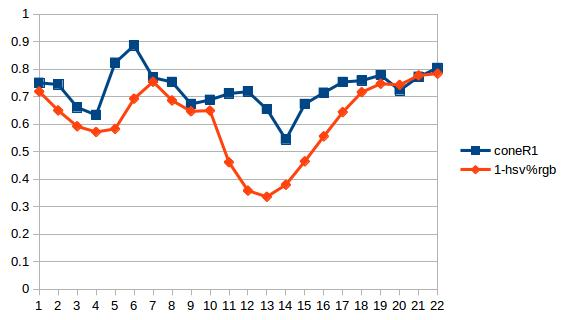
\includegraphics[width=1\linewidth]{figures/correlations/rgb/room_hsv.jpg}
  \caption{}
\end{subfigure}
\hfill
\begin{subfigure}{.49\linewidth}
  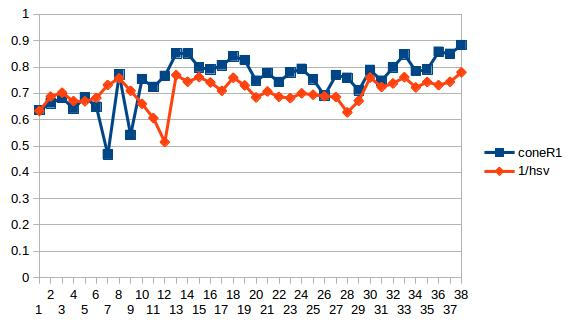
\includegraphics[width=1\linewidth]{figures/correlations/db/campus_hsv.jpg}
  \caption{}
\end{subfigure}
\begin{subfigure}{.49\linewidth}
  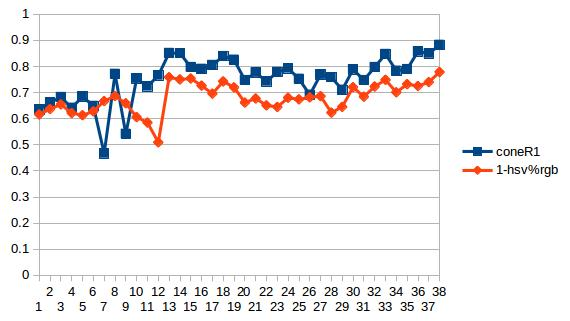
\includegraphics[width=1\linewidth]{figures/correlations/rgb/campus_hsv.jpg}
  \caption{}
\end{subfigure}
\hfill
\begin{subfigure}{.49\linewidth}
  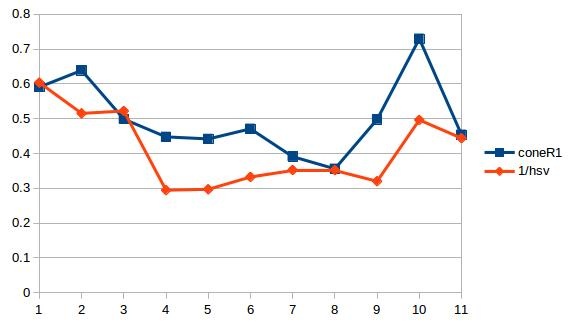
\includegraphics[width=1\linewidth]{figures/correlations/db/pets2_hsv.jpg}
  \caption{}
\end{subfigure}
\begin{subfigure}{.49\linewidth}
  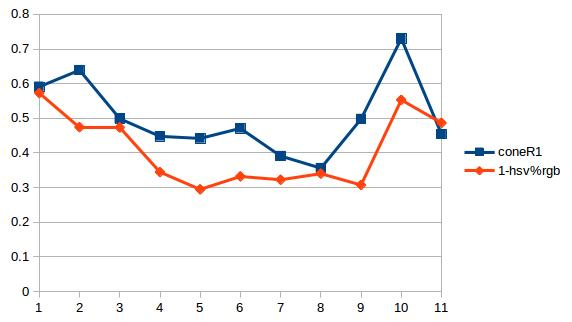
\includegraphics[width=1\linewidth]{figures/correlations/rgb/pets2_hsv.jpg}
  \caption{}
\end{subfigure}

\caption{Comparison of dB and \%$\Delta$ models of attenuation. }
\label{fig:corr_compare}
\end{figure}

\subsection{Correlation Improvements}
\subsubsection{Low-contrast Keypoints}
\textit{Correlation: coneR1 avgAtten*lowcSat}

%%%
\section{Brightness Models}
%%%

In addition to attenuation models, datasets also respond uniquely to varying brightness models. Figure \ref{fig:brightness_example} visualizes the disparity between multiple modes of brightness calculation, and how it may affect the correlation coefficient of attenuation. Tables \ref{table:brightness_corr_db} and \ref{table:brightness_corr_rgb} enumerate the correlative changes experienced by each dataset when subjected to multiple modes of brightness calculation.

% example 
\begin{figure}
\centering
\begin{subfigure}{.49\linewidth}
  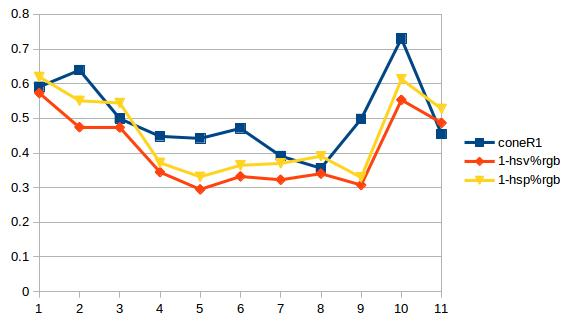
\includegraphics[width=1\linewidth]{figures/brightness/rgb/pets2_hsv_hsp.jpg}
  \caption{PETS2}
\end{subfigure}
\hfill
\begin{subfigure}{.49\linewidth}
  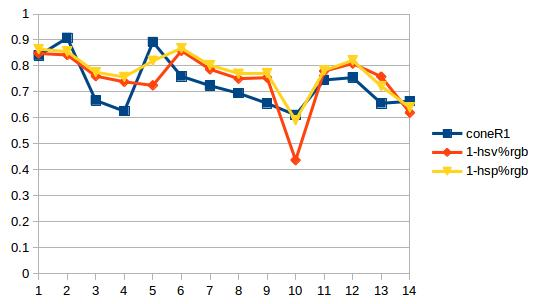
\includegraphics[width=1\linewidth]{figures/brightness/rgb/lab_hsv_hsp.jpg}
  \caption{aton\_lab}
\end{subfigure}

\caption{Example contrasting correlation improvements of the \%$\Delta$-HSP model (yellow) against \%$\Delta$-HSV (red) and optimal \textit{coneR1} (blue). }
\label{fig:brightness_example}
\end{figure}

% Table Form ((dB) Corr v. Brightness
\begin{sidewaystable}
\begin{tabular}{ |c|c|c|c|c|c|c|c| }
	\hline
	\textbf{Dataset} & \textbf{HSV} & \textbf{HSP} & \textbf{HSI} & \textbf{HSL}& \textbf{Y'} & \textbf{Norm} \\
	\hline
	\hline
	\textbf{PETS1} & 0.1985540659 & 0.2267703534 & 0.2021748353 & 0.1896175839 & 0.2221548898 & 0.2046326852 \\
	\hline
	\textbf{PETS2} & 0.6705816077 & 0.7057667571 & 0.6896919047 & 0.6532729231 & 0.6957362604 & 0.6945302273 \\
	\hline
	\textbf{aton\_highway1} & 0.683685054 & 0.4771690254 & 0.5235779189 & 0.5604481428 & 0.4707739954 & 0.6694458799 \\
	\hline
	\textbf{aton\_highway3} & 0.7424117824 & 0.8141308312 & 0.7946054861 & 0.7801949863 & 0.8158763583 & 0.7732651826 \\
	\hline
	\textbf{aton\_room} & 0.5477587003 & 0.5284545338 & 0.5324865293 & 0.5361978128 & 0.5274008032 & 0.531798353 \\
	\hline
	\textbf{aton\_campus} & 0.3599691597 & 0.4828464391 & 0.4304907395 & 0.4163027706 & 0.486961905	 & 0.4199883154 \\
	\hline
	\textbf{aton\_hallway} & 0.6561589554 & 0.6253115335 & 0.6174353175 & 0.622359453 & 0.6177818392 & 0.6014888237 \\
	\hline
	\textbf{aton\_lab} & 0.6954036581 & 0.709605239 & 0.7047840902 & 0.7174673715 & 0.7100507268 & 0.7078891946 \\
	\hline
\end{tabular}
\caption{Datasets and their correlations to \textit{coneR1} (dB attenuation model) against Brightness models.}
\label{table:brightness_corr_db}
\end{sidewaystable}

% Brightness Models (dB)
%\begin{figure}
\begin{sidewaysfigure}
  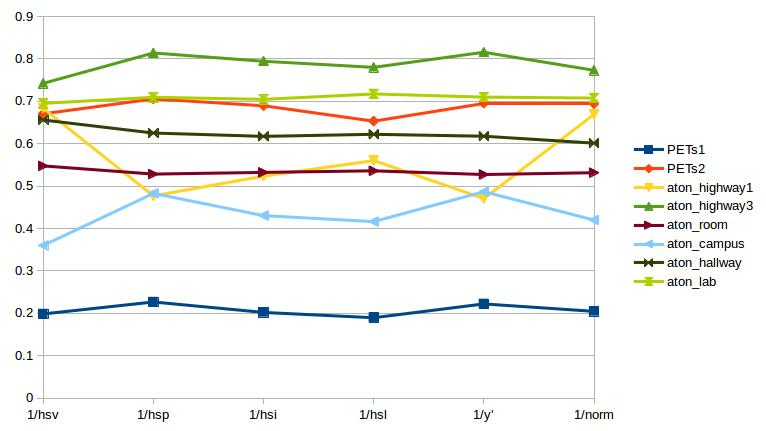
\includegraphics[width=\linewidth]{figures/brightness/db/correlation_x.jpg}
  \caption{\textbf{REMOVE W3C!}}
\label{fig:brightness_corr_db}
%\end{figure}
\end{sidewaysfigure}

% Table Form (RGB) Corr v. Brightness
\begin{sidewaystable}
\begin{tabular}{ |c|c|c|c|c|c|c|c| }
	\hline
	\textbf{Dataset} & \textbf{HSV} & \textbf{HSP} & \textbf{HSI} & \textbf{HSL}& \textbf{Y'} & \textbf{Norm} \\
	\hline
	\hline
	\textbf{PETS1} & 0.1837705578 & 0.3195109707 & 0.2409348587 & 0.2221233609 & 0.23915228 & 0.313683891 \\
	\hline
	\textbf{PETS2} & 0.7430874979 & 0.74107993 & 0.7457147971 & 0.7171166185 & 0.7477276409 & 0.7321917683 \\
	\hline
	\textbf{aton\_highway1} & 0.5923176614 & 0.189234362 & 0.3938107273 & 0.3963106037 & 0.3130064246 & 0.2163996242 \\
	\hline
	\textbf{aton\_highway3} & 0.8013856844 & 0.7617161728 & 0.8043846426 & 0.7817768177 & 0.8154623374 & 0.7601502706 \\
	\hline
	\textbf{aton\_room} & 0.6226957045 & 0.6182383922 & 0.6213184407 & 0.6216344105 & 0.6232803965 & 0.6168184555 \\
	\hline
	\textbf{aton\_campus} & 0.5645999518 & 0.3715622333 & 0.4071502522 & 0.3954402236 & 0.4594624596 & 0.3611939942 \\
	\hline
	\textbf{aton\_hallway} & 0.6897315501 & 0.4291871503 & 0.7461485549 & 0.7539042742 & 0.7563870311 & 0.4042302237 \\
	\hline
	\textbf{aton\_lab} & 0.5508747537 & 0.729256455 & 0.5919609092 & 0.6083788718 & 0.5978292247 & 0.7252228893 \\
	\hline
\end{tabular}
\caption{Datasets and their correlations to \textit{coneR1} (\%$\Delta$ attenuation model) against Brightness models.}
\label{table:brightness_corr_rgb}
\end{sidewaystable}

% Brightness Models (RGB)
\begin{sidewaysfigure}
  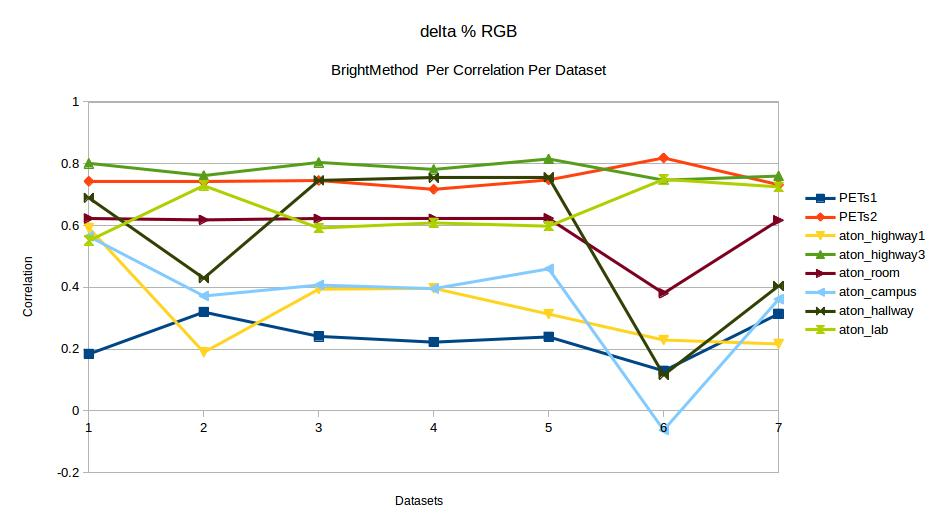
\includegraphics[width=\linewidth]{figures/brightness/rgb/correlation_x.jpg}
  \caption{\textbf{REMOVE W3C!}}
\label{fig:brightness_corr_rgb}
\end{sidewaysfigure}

Two distinct response trends are observed in Figure \ref{fig:brightness_corr_db}. These trends are clearly shown in Figure \ref{fig:brightness_indoor_outdoor}: outdoor datasets (PETS1, PETS2, highway3, and campus) share a similar response to changing brightness models, while indoor datasets (room, hallway, and lab) also share a similar response. The difference in brightness models can be primarily characterized by their individual treatments of color content in a pixel. The grouping of datasets further reinforces the importance of color shift depending on the environment.

The exception to this grouping of outdoor and indoor datasets is aton\_highway1, an outdoor dastaset that has a response reciprocal to that of most outdoor environments. Figure \ref{fig:highway1_reciprocal} visualizes the mirrored nature of aton\_highway1's response. In Chapter \textbf{METHODOLOGY} in section \textbf{WOOWOO}, we can see aton\_highway1's RGB shift in shadowed regions (figure reference?). The RGB shift is characteristic of an outdoor scene; red, green, and blue channels were attenuated by different amounts. However, aton\_highway1 contains the darkest cast shadows in relation to its background model. The highest of aton\_highway1's responses, HSV and Norm, both result in an over-valued brightness value in accordance to color shifts. While these serve as relative low points in other outdoor datasets for that reason, the larger calculated brightness attenuation simply provided for a closer relational value with the optimal \textit{coneR1} value in the dark shadowed region.

% Brightness Models indoor/outdoor (dB)
\begin{figure}
\centering
\begin{subfigure}{.8\linewidth}
  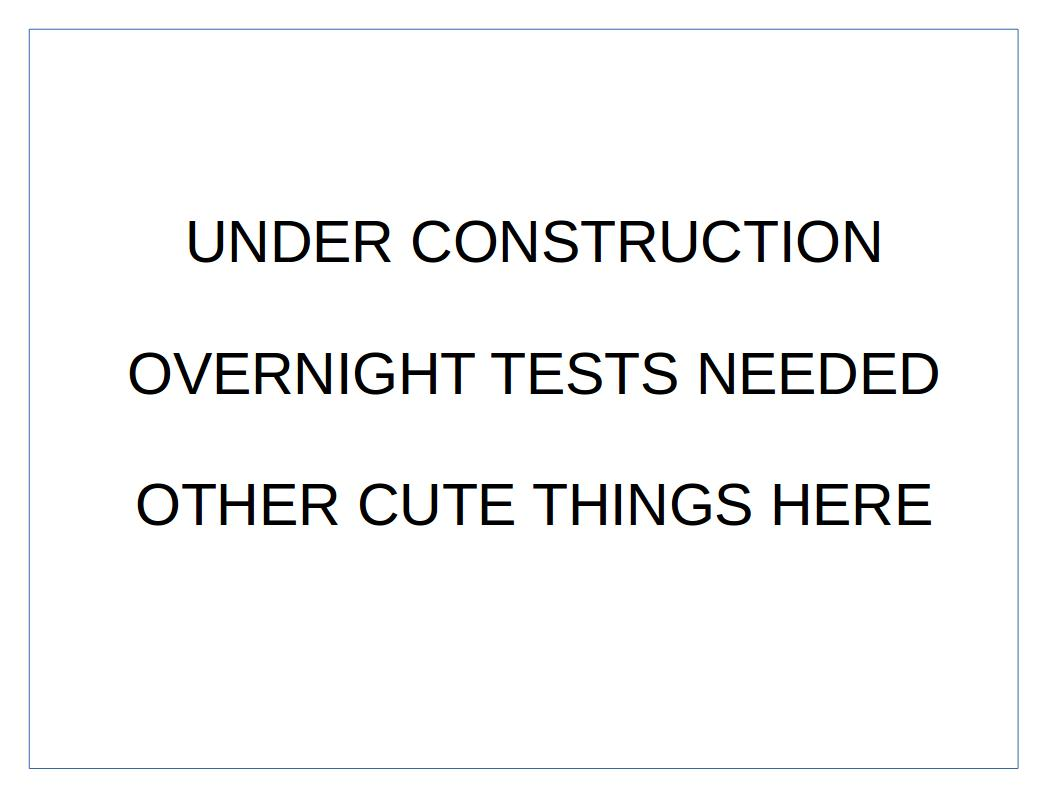
\includegraphics[width=1\linewidth]{figures/placeholder.jpg}
  \caption{}
\end{subfigure}
\hfill
\begin{subfigure}{.8\linewidth}
  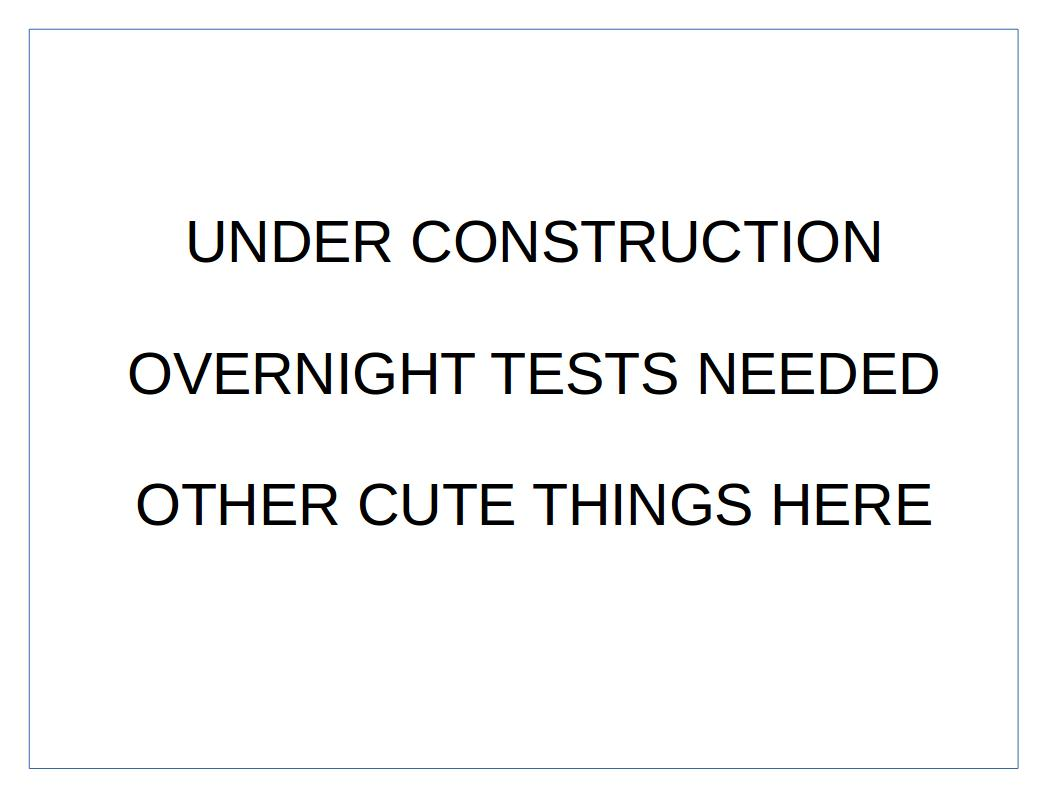
\includegraphics[width=1\linewidth]{figures/placeholder.jpg}
  \caption{}
\end{subfigure}

\caption{Outdoor datasets (a) share a common response to varying brightness models. In contrast, indoor datasets (b) share a common lack of response.}
\label{fig:brightness_indoor_outdoor}
\end{figure}

% Aton_highway1 oddity
\begin{figure}
\centering
  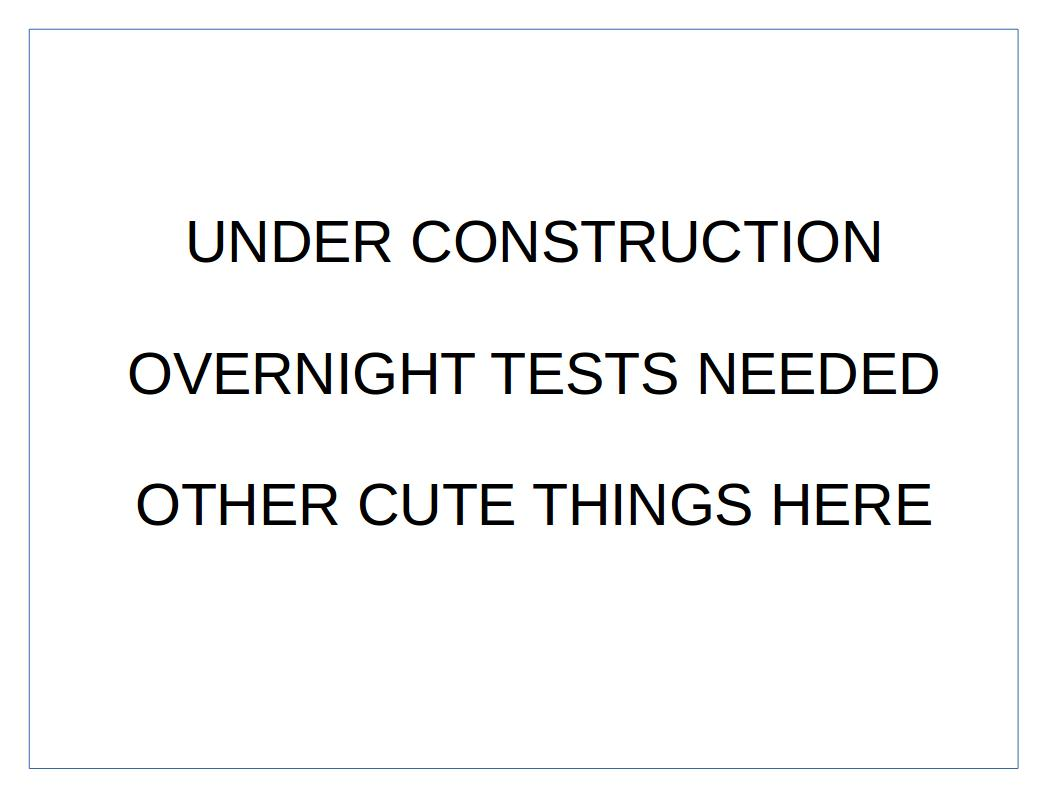
\includegraphics[width=.7\linewidth]{figures/placeholder.jpg}
\caption{aton\_highway1's response to various brightness models is foil to other outdoor datasets' responses.}
\label{fig:highway1_reciprocal}
\end{figure}

%%%
\section{Parameter Model Results}
%%%
% RGB shift per req. shift to optimal
\begin{figure}
\centering
\begin{subfigure}{.49\linewidth}
  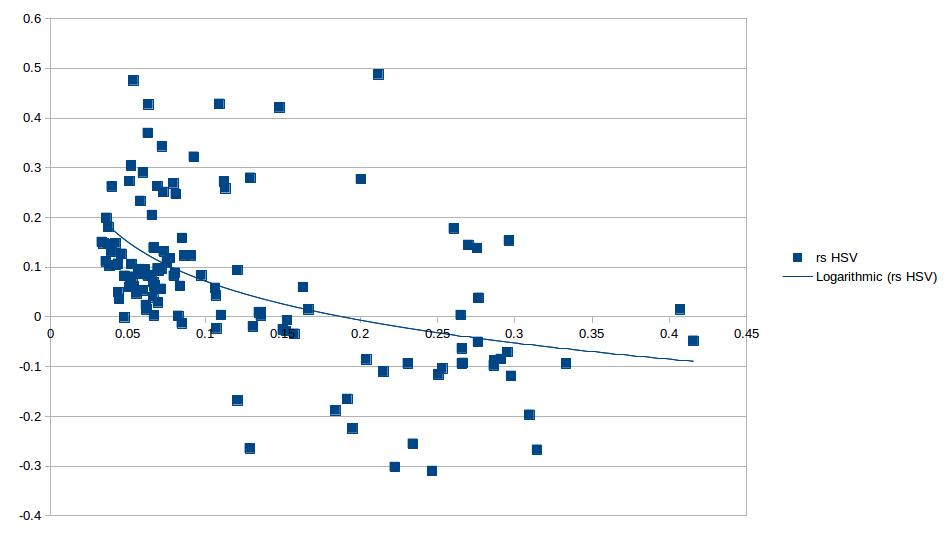
\includegraphics[width=1\linewidth]{figures/model_hsv.jpg}
  \caption{HSV}
\end{subfigure}
\hfill
\begin{subfigure}{.49\linewidth}
  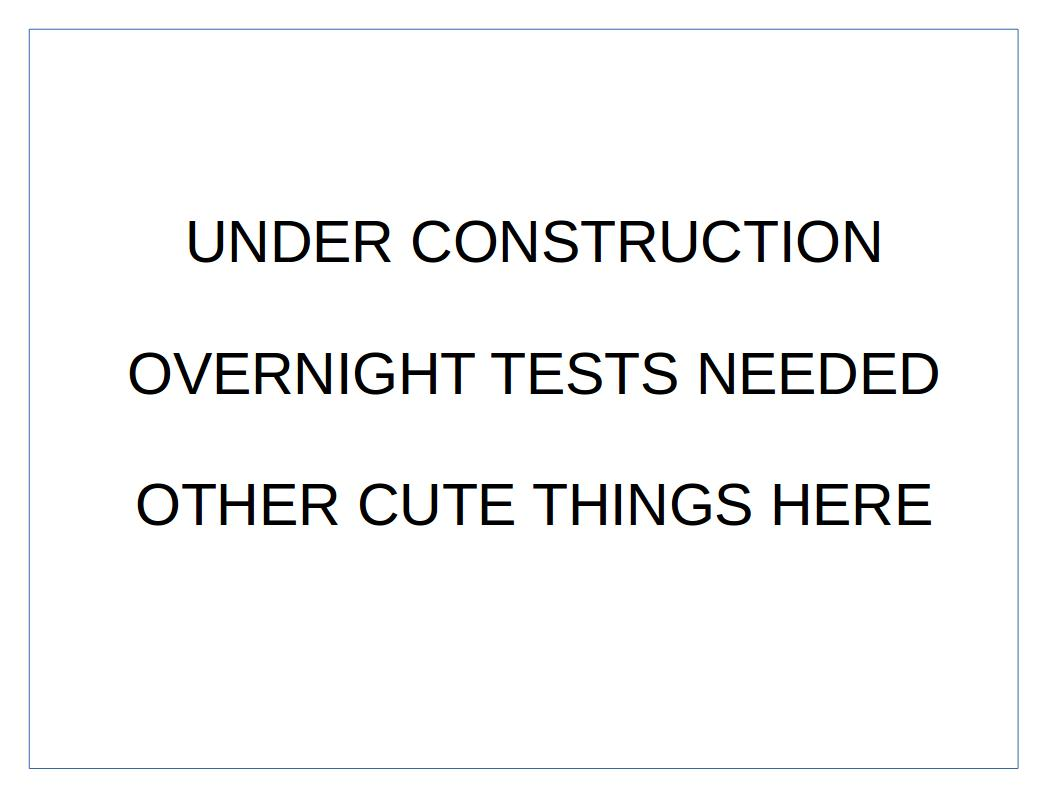
\includegraphics[width=1\linewidth]{figures/placeholder.jpg}
  \caption{HSP}
\end{subfigure}
\hfill
\begin{subfigure}{.49\linewidth}
  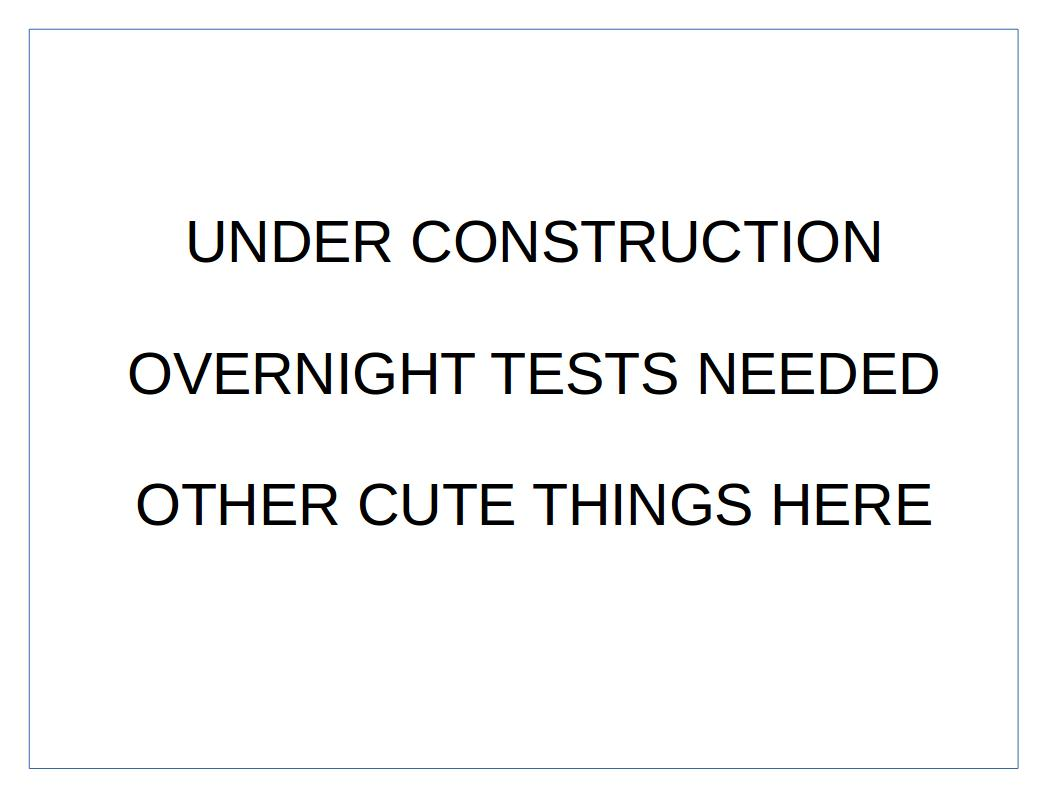
\includegraphics[width=1\linewidth]{figures/placeholder.jpg}
  \caption{HSI}
\end{subfigure}
\hfill
\begin{subfigure}{.49\linewidth}
  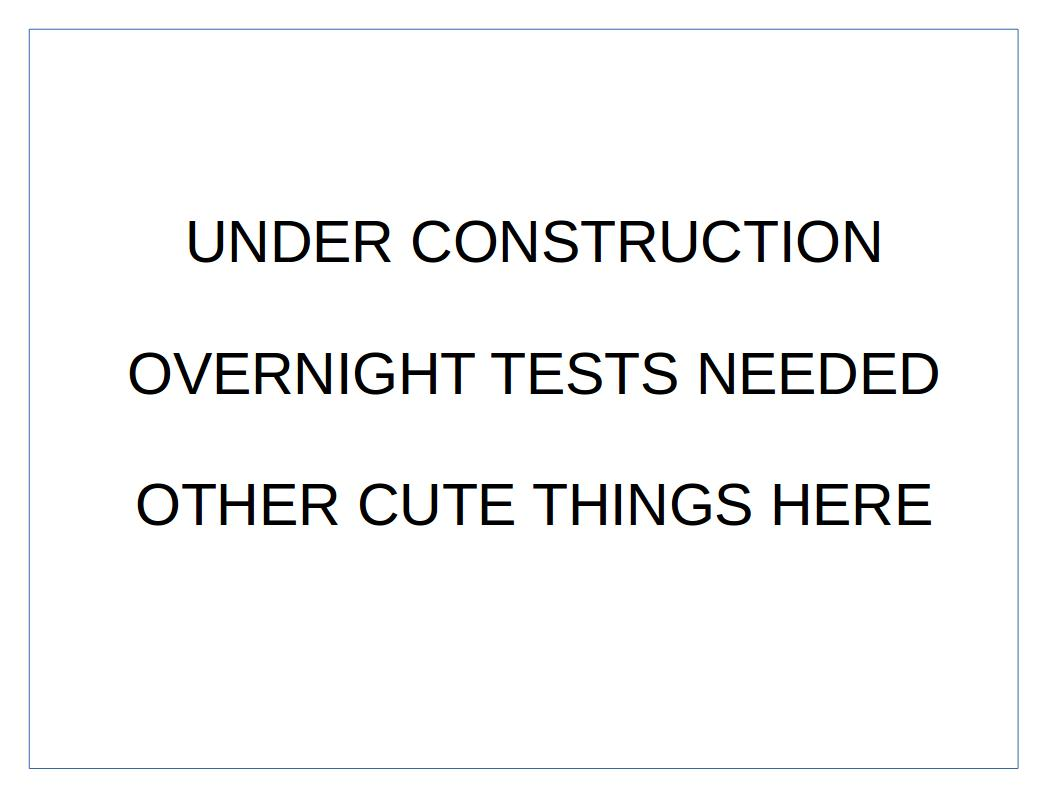
\includegraphics[width=1\linewidth]{figures/placeholder.jpg}
  \caption{HSL}
\end{subfigure}
\hfill
\begin{subfigure}{.49\linewidth}
  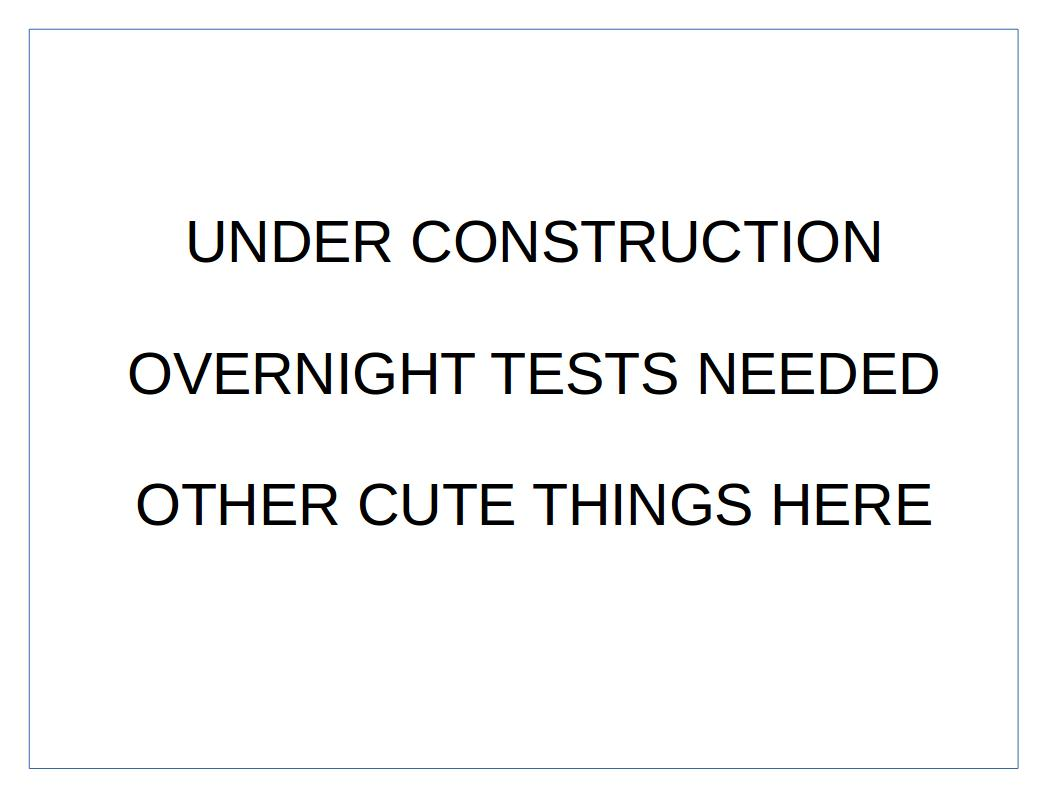
\includegraphics[width=1\linewidth]{figures/placeholder.jpg}
  \caption{Luma (Y')}
\end{subfigure}
\hfill
\begin{subfigure}{.49\linewidth}
  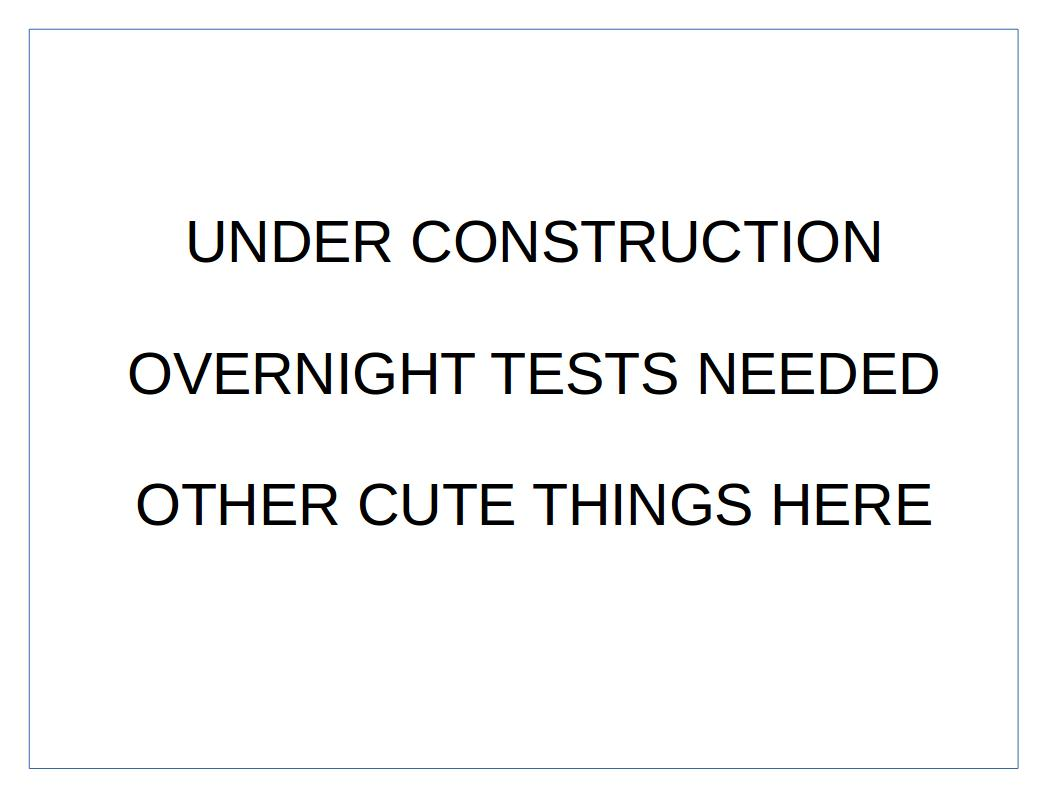
\includegraphics[width=1\linewidth]{figures/placeholder.jpg}
  \caption{Norm}
\end{subfigure}

\caption{Outdoor datasets (a) share a common response to varying brightness models. In contrast, indoor datasets (b) share a common lack of response.}
\label{fig:brightness_indoor_outdoor}
\end{figure}

% detect/discrim calc
\begin{figure}
\centering
\begin{subfigure}{1\linewidth}
  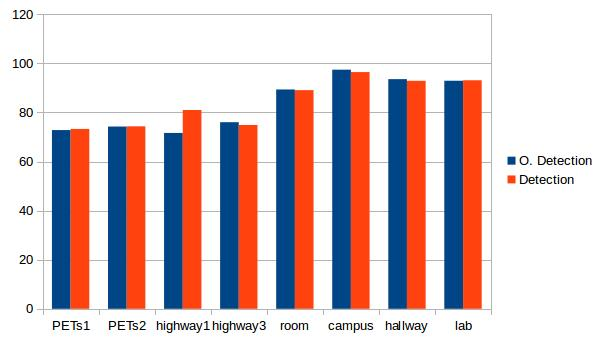
\includegraphics[width=1\linewidth]{figures/model/detect_hsv.jpg}
  \caption{}
\end{subfigure}
\hfill
\begin{subfigure}{1\linewidth}
  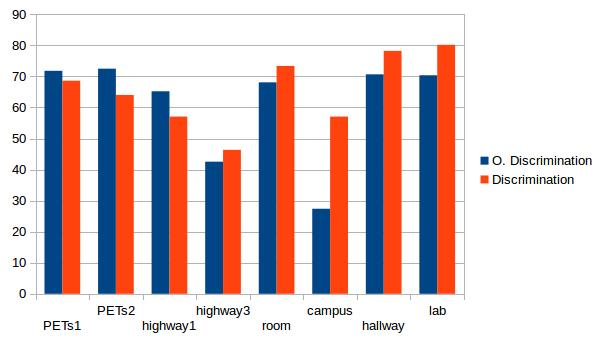
\includegraphics[width=1\linewidth]{figures/model/discrim_hsv.jpg}
  \caption{}
\end{subfigure}

\caption{Detection (a) and Discrimination (b) calculated using the HSV parameter model, for each dataset.}
\label{fig:bars_hsv_calc}
\end{figure}

% HSV, HSP, etc for one dataset
\begin{figure}
\centering
  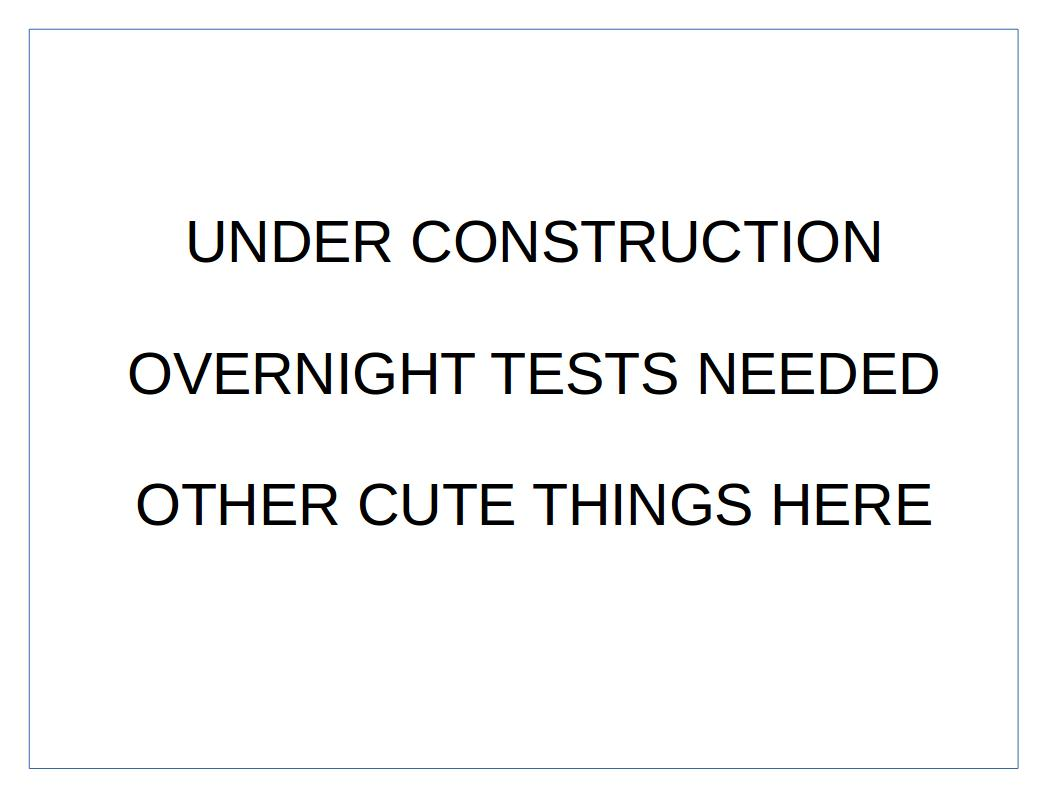
\includegraphics[width=1\linewidth]{figures/placeholder.jpg}
\caption{Detection (blue) and Discrimination (orange) for each brightness model. Dataset: PETS1. Full results for all datasets can be found in the appendix.}
\label{fig:pets1_bars_calc_all}
\end{figure}

\end{document}
